\chapter{相近题型辨析}
\section{同样是极限}
\begin{tabularx}{\textwidth}{p{29mm}Y Y}
\toprule 结构&优先方法&第一步怎么写\\\midrule
乘除，无主项抵消&等价无穷小&先确认每一项趋于0，整体可拆为有限个比值。\\
相减，两项同阶&泰勒定阶&通分后看抵消，展开到首个不相消的项；$\sin x-x\sim-x^3/6$。\\
$u(x)^{v(x)}$&对数化&写$\ln y=v\ln u$；底数须为正，再判断对数式极限。\\
$f(a+h)-f(a)$&导数定义&先找实际增量$h$，乘除$h$；只知可导时用$f(a+h)=f(a)+f'(a)h+o(h)$。\\
积分趋零&积分定阶&$\varphi(t)\sim ct^p$且$p>-1$时，$\int_0^u\varphi(t)dt\sim cu^{p+1}/(p+1)$。\\
含未知函数且仅知连续&从极限剥离&先逼出函数值，再将原条件改成差商；不对未知函数直接洛必达。\\\bottomrule
\end{tabularx}
\tip{定阶要包含外层}{比较$\int_0^{x^2}(e^{t^3}-1)dt$与$x^7$：被积函数主项$t^3$，积分是$u^4/4$，上限$u=x^2$使结果为$x^8/4$。完整链为“内层3阶，积分加1，上限乘2”。}

\section{同样是导数条件}
\begin{tabularx}{\textwidth}{p{33mm}Y}
\toprule 条件或目标&应检查的对象\\\midrule
一元函数在接点可导&函数值先接上，分别算左右差商；邻域内导数公式不能直接代接点。\\
一元导数连续&先证明接点可导，再比较邻域导数极限与接点导数值。\\
极值候选点&可导内点有$f'=0$；还要看导数变号，$x^3$在0导数为0但无极值。\\
拐点候选点&看凹凸是否变换，$f''=0$只是候选；$x^4$在0不是拐点。\\
二元偏导存在&只沿坐标方向作差商，不代表所有方向变化可控。\\
二元可微&检验$f(x_0+h,y_0+k)-f_0-Ah-Bk=o(\sqrt{h^2+k^2})$。\\\bottomrule
\end{tabularx}
\core{振荡函数的三道门：$f(x)=x^\alpha\sin(x^{-\beta})$（$x>0$），$f(0)=0$，$\alpha,\beta>0$。连续由$|f(x)|\le x^\alpha$；右差商趋零需$\alpha>1$；导数中最强振荡项为$-\beta x^{\alpha-\beta-1}\cos(x^{-\beta})$，导数右连续需$\alpha>\beta+1$。每提升一个目标，就重新估计实际出现的幂次。}
\tip{偏导存在仍不可微}{令$f(x,y)=xy/\sqrt{x^2+y^2}$（非原点），原点取0。两偏导均为0，且$|f|\le\sqrt{x^2+y^2}/2$故连续；但沿$x=y=t>0$，$f/\sqrt{x^2+y^2}=1/2$，线性余项不趋零，所以不可微。}

\section{同样是积分}
\begin{tabularx}{\textwidth}{p{27mm}Y Y}
\toprule 任务&识别结构&最短入口\\\midrule
求原函数&多项式乘指数/三角&分部积分降低多项式次数。\\
有理式积分&分母可因式分解&先长除，再部分分式；二次不可约项配成导数项加反正切。\\
定积分求值&上下限互补、对称&试$x\mapsto a+b-x$，相加看是否消去难因子。\\
定积分比较&权重相同/区间相同&比较被积函数；变号时先分段，不能整体套不等式。\\
二重积分&内积分难、区域简单&换序；圆与径向函数出现时用极坐标。\\
反常积分&端点奇异或无穷&先分端点判敛散，再求值，最后取各条件交集。\\\bottomrule
\end{tabularx}
\core{端点幂次的方向相反：$\int_0^1 x^{-p}dx$收敛要求$p<1$；$\int_1^\infty x^{-p}dx$收敛要求$p>1$。例如$\arctan x/[x^p(1+x)]$在0等价$x^{1-p}$，在无穷等价$(\pi/2)x^{-p-1}$，两端合并为$0<p<2$。}

\section{先画域再换元}
\begin{center}
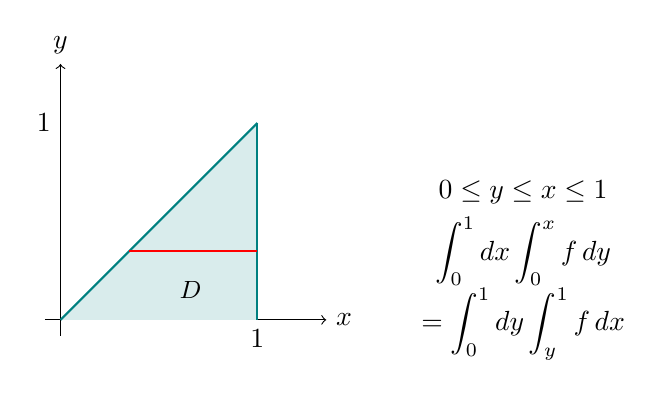
\begin{tikzpicture}[scale=2.5]
\draw[->] (-.08,0)--(1.35,0) node[right]{$x$};\draw[->] (0,-.08)--(0,1.3) node[above]{$y$};
\fill[teal!15] (0,0)--(1,1)--(1,0)--cycle;
\draw[teal,thick] (0,0)--(1,1);\draw[teal,thick] (1,0)--(1,1);
\draw[red,thick] (.35,.35)--(1,.35);\node at (.66,.15){\small $D$};
\node[left] at (0,1){$1$};\node[below] at (1,0){$1$};
\node at (2.35,.65){$0\le y\le x\le1$};\node at (2.35,.35){$\displaystyle\int_0^1dx\int_0^x f\,dy$};
\node at (2.35,-.02){$\displaystyle=\int_0^1dy\int_y^1 f\,dx$};
\end{tikzpicture}
\end{center}
横切线固定$y$，进入点是$x=y$、离开点是$x=1$。换序的核心是换一种切片，而不是交换积分号后的字母。
\begin{tabularx}{\textwidth}{p{35mm}Y}
\toprule 题面线索&选择依据\\\midrule
$x^2+y^2$与圆、扇形&极坐标把径向表达式化为$r$，面积元必须乘$r$。\\
$xy=c$和$y=kx$&试$u=xy,v=y/x$，四条边变常数；也可先用交换对称消项再算面积。\\
$x+y$与$x-y$平行线&线性换元使斜矩形变矩形，雅可比取绝对值。\\
区域关于$x=y$对称&$\iint_Df(x,y)=\iint_Df(y,x)$；$(x-y)$消去，$(x-y)^2$不消去。\\
区域是交集&每个方向取更严格边界；两圆极坐标上界往往是$\min\{a\cos\theta,b\sin\theta\}$，须在交角处分段。\\\bottomrule
\end{tabularx}

\section{证明从目标倒推}
\begin{tabularx}{\textwidth}{p{39mm}Y}
\toprule 目标形状&构造方向\\\midrule
$f'(\xi)=\frac{f(b)-f(a)}{b-a}$&拉格朗日；端点差商已经把区间告诉你。\\
$f'(\xi)g(\xi)-f(\xi)g'(\xi)=0$&先试$(f/g)'$，检查$g\ne0$；或柯西中值。\\
$f'(\xi)+cf(\xi)=0$&积分因子：$(e^{cx}f(x))'$。\\
$f''(\xi)=C$&构造$f$减二次多项式，使三个零点成立，连续两次罗尔。\\
$|f-L|\le M(x-a)(b-x)/2$&减端点插值直线$L$，用二阶导界；控制曲线与弦的误差。\\
积分与函数值比较&先看凸性、单调性或积分中值；必要性常把区间缩小再泰勒展开。\\\bottomrule
\end{tabularx}
\tip{辅助函数不是靠猜}{若要$f'(\xi)=f(\xi)/(2-\xi)$，把式子移到一边为$(2-\xi)f'(\xi)-f(\xi)=0$，它正是$[(2-x)f(x)]'=0$。先识别乘积导数，再检查两个端点值能否相等。}

\section{三种矩阵变换}
\begin{tabularx}{\textwidth}{p{37mm}p{34mm}Y}
\toprule 关系&保持什么&解题动作\\\midrule
等价 $B=PAQ$&秩&阶梯形；只问存在可逆左右因子时比秩。\\
相似 $B=P^{-1}AP$&特征多项式、特征值、迹、行列式&按目标对角元素排列特征向量；重根另查特征子空间维数。\\
合同 $B=P^TAP$&实对称阵正负惯性指数&配方或惯性；特征值的数值通常不保持。\\
正交合同 $B=Q^TAQ$&同时是相似，保特征值&实对称阵特征分解，向量正交单位化。\\\bottomrule
\end{tabularx}
\tip{同号不等于同特征值}{$A=\operatorname{diag}(1,2,0)$与$B=\operatorname{diag}(3,7,0)$均有两个正惯性指数、秩2，所以合同；特征值集合不同，所以不相似。取$P=\operatorname{diag}(\sqrt3,\sqrt{7/2},1)$即可验证$P^TAP=B$。}
\core{低秩幂：若$A=GH$，其中$G$为$n\times r$、$H$为$r\times n$，则$A^k=G(HG)^{k-1}H$。例如$A=uv^T$有$A^k=(v^Tu)^{k-1}uv^T$。题目给极大无关列且要求高次幂时，先把其余列写成它们的组合，往往比求$n$阶特征多项式更短。}

\section{公式落地检查}
\begin{itemize}
\item 泰勒：展开点一致、阶数够用、余项在除法后仍趋零。
\item 求导：变量依赖完整；参数二阶导要再除一次$x'(t)$；隐函数先检查分母非零。
\item 积分：积分变量、范围、微元、变限后的符号全部同时改变。
\item 几何：垂直旋转轴的截面有孔时，用外半径平方减内半径平方；面积与有向积分分清。
\item 方程：齐次解与非齐次特解的叠加系数条件不同；共振要乘足够次$x$。
\item 线代：矩阵乘法不交换；伴随先判可逆；公共解先数维数；正交变换向量要单位化。
\end{itemize}
